\scanpage{128}
sait que les traces d'endomorphismes des modules de type fini sur le dit $\Lambda$ sont \unsure{définis} --- et la formule de Lefschetz \unsure{(*)} permettra bien de vérifier un \inserted{\unsure{provenant de}\illegible{1}} \unsure{$\ell$-adique} est un véritable \uline{entier}. Cependant, on a envie de dire que cette formule de Lefschetz n'est que la conséquence formelle, par passage à la limite, des formules de Lefschetz qu'on va écrire pour chacun \inserted{des} anneaux de coeff. $\mathbb Z/\ell^\nu\mathbb Z$.

Comme d'habitude, pour écrire une formule correcte (pour un $A=\mathbb Z/N\mathbb Z$ \uline{donné}) il y a lieu de remplacer le système des $H^i(X,A_X)$ (disons) par le \uline{complexe} \inserted{$\mathbb R\Gamma_X(\Lambda_X)$} qui lui donne naissance, et le système des $f^{(i)}$ par l'endomorphisme $\mathbb R\Gamma_X(f)$ de ce complexe défini ``par \unsure{fonctorialité}''.

\figure{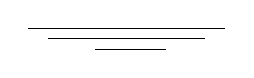
\begin{tikzpicture}\draw (0,0)--(2.5,0);\draw (.25,-.13)--(2.25,-.13);\draw (.85,-.27)--(1.75,-.27);\end{tikzpicture}}

Pour ceci, considérons de façon générale un complexe $L_\bullet$ sur un anneau comm. $A$
\mspage{127}
